\section{Présentation générale}

\subsection{Entreprise}
\subsubsection{Histoire d'Amazon}
\paragraph{}
\vspace{-2em}  % 减少1em的垂直空间
Amazon (NASDAQ: AMZN) est une multinationale américaine basée à Seattle.

\paragraph{}
\vspace{-2em}  % 减少1em的垂直空间
Fondée par Jeff Bezos en 01 juillet 1994, 
l'entreprise a été introduite en Bourse au NASDAQ en 01 mai 1997.
\paragraph{}
\vspace{-2em}  % 减少1em的垂直空间
L'activité initiale de la société Amazon concernait la vente à distance de livres, avant que la société ne se diversifie dans la vente en ligne de produits culturels et marchands, profitant de l'explosion d'internet.
\paragraph{}
\vspace{-2em}  % 减少1em的垂直空间
Progressivement, le groupe se lance agressivement dans de nombreux domaines comme l'informatique, la grande distribution, la production cinématographique, les objets connectés, les cliniques de santé, ou l'industrie militaire.
\paragraph{}
\vspace{-2em}  % 减少1em的垂直空间
C'est un des géants du Web, regroupés sous l'acronyme GAFAM.


\begin{figure}[htbp]
    %\begin{subfigure}{0.5\textwidth}
        \centering
        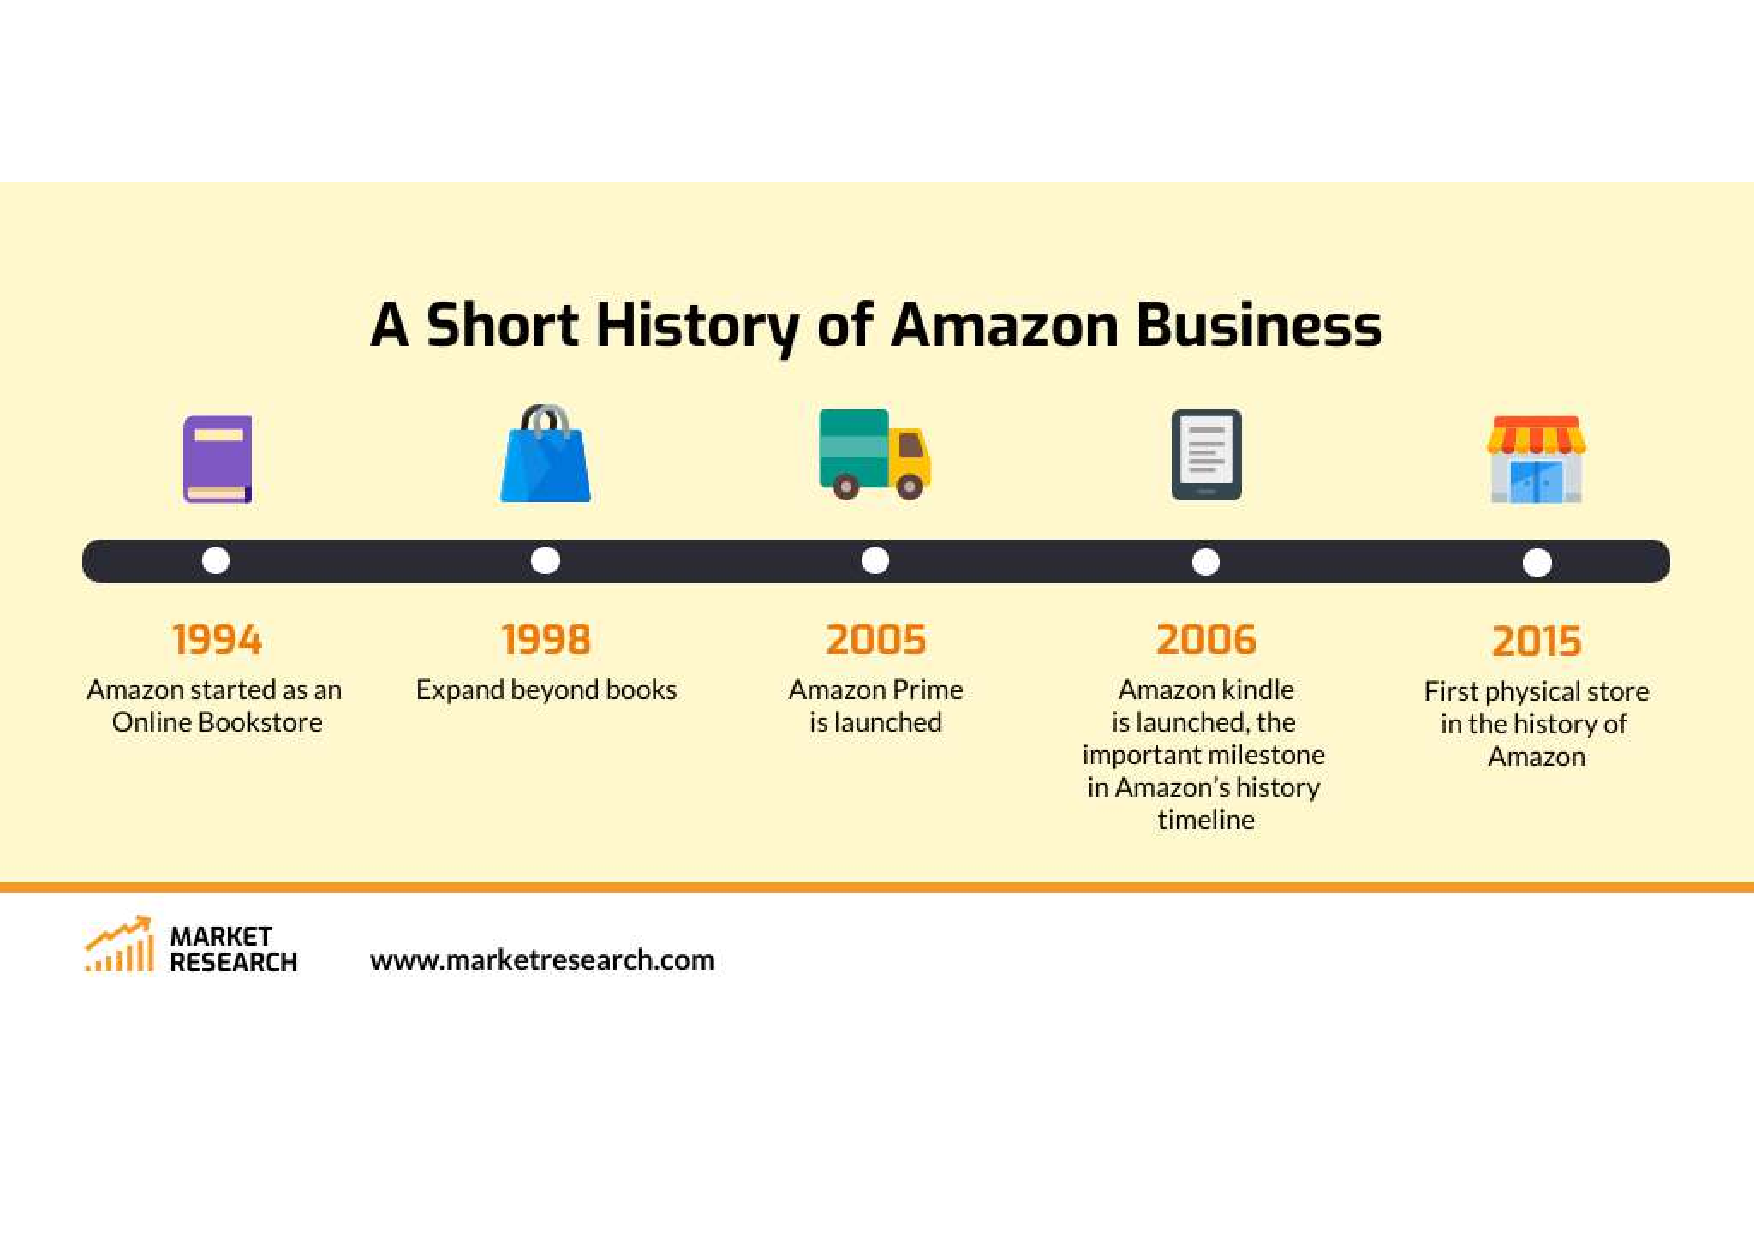
\includegraphics[width=0.8\linewidth]{./Graphismes-UTC/logos/Amazon/history.pdf}\hfill
        %\vspace{-1em}
        \caption{L'Histoire d'Amazon}
    \end{figure}

\paragraph{}
\vspace{-2em}  % 减少1em的垂直空间
\subsubsection{Domaines d'activité et ses compétences}
Amazon, initialement fondé comme une simple plateforme de commerce électronique, a rapidement évolué bien au-delà de ses débuts modestes.
\paragraph{}
\vspace{-2em}  % 减少1em的垂直空间
\begin{itemize}
    \item Commerce Électronique :
    \begin{itemize}
        \item Plateforme exhaustive offrant une vaste gamme de produits.
        \item Interface conviviale facilitant la navigation et les achats en ligne.
    \end{itemize}

    \item Logistique Efficace :
    \begin{itemize} 
        \item Réseau mondial d'entrepôts et de centres de distribution.
        \item Livraison rapide et fiable grâce à une chaîne d'approvisionnement bien organisée.
    \end{itemize}

    \item Amazon Web Services (AWS) :
    \begin{itemize}
        \item Leader mondial du cloud computing.
        \item Offre des solutions de pointe en matière de stockage, de traitement de données et d'intelligence artificielle.
    \end{itemize}

    \item Services d'Abonnement (Amazon Prime) :
    \begin{itemize}
        \item Avantages exclusifs tels que la livraison express gratuite.
        \item Accès à une variété de contenus multimédias, y compris des séries, des films et de la musique.
    \end{itemize}

    \item Marketplace pour Vendeurs Tiers :
    \begin{itemize}
        \item Plateforme permettant à des milliers de petites entreprises de vendre leurs produits.
        \item Favorise une communauté diversifiée d'entreprises et d'entrepreneurs.
    \end{itemize}
\end{itemize}

\begin{figure}[htbp]
    %\begin{subfigure}{0.5\textwidth}
        \centering
        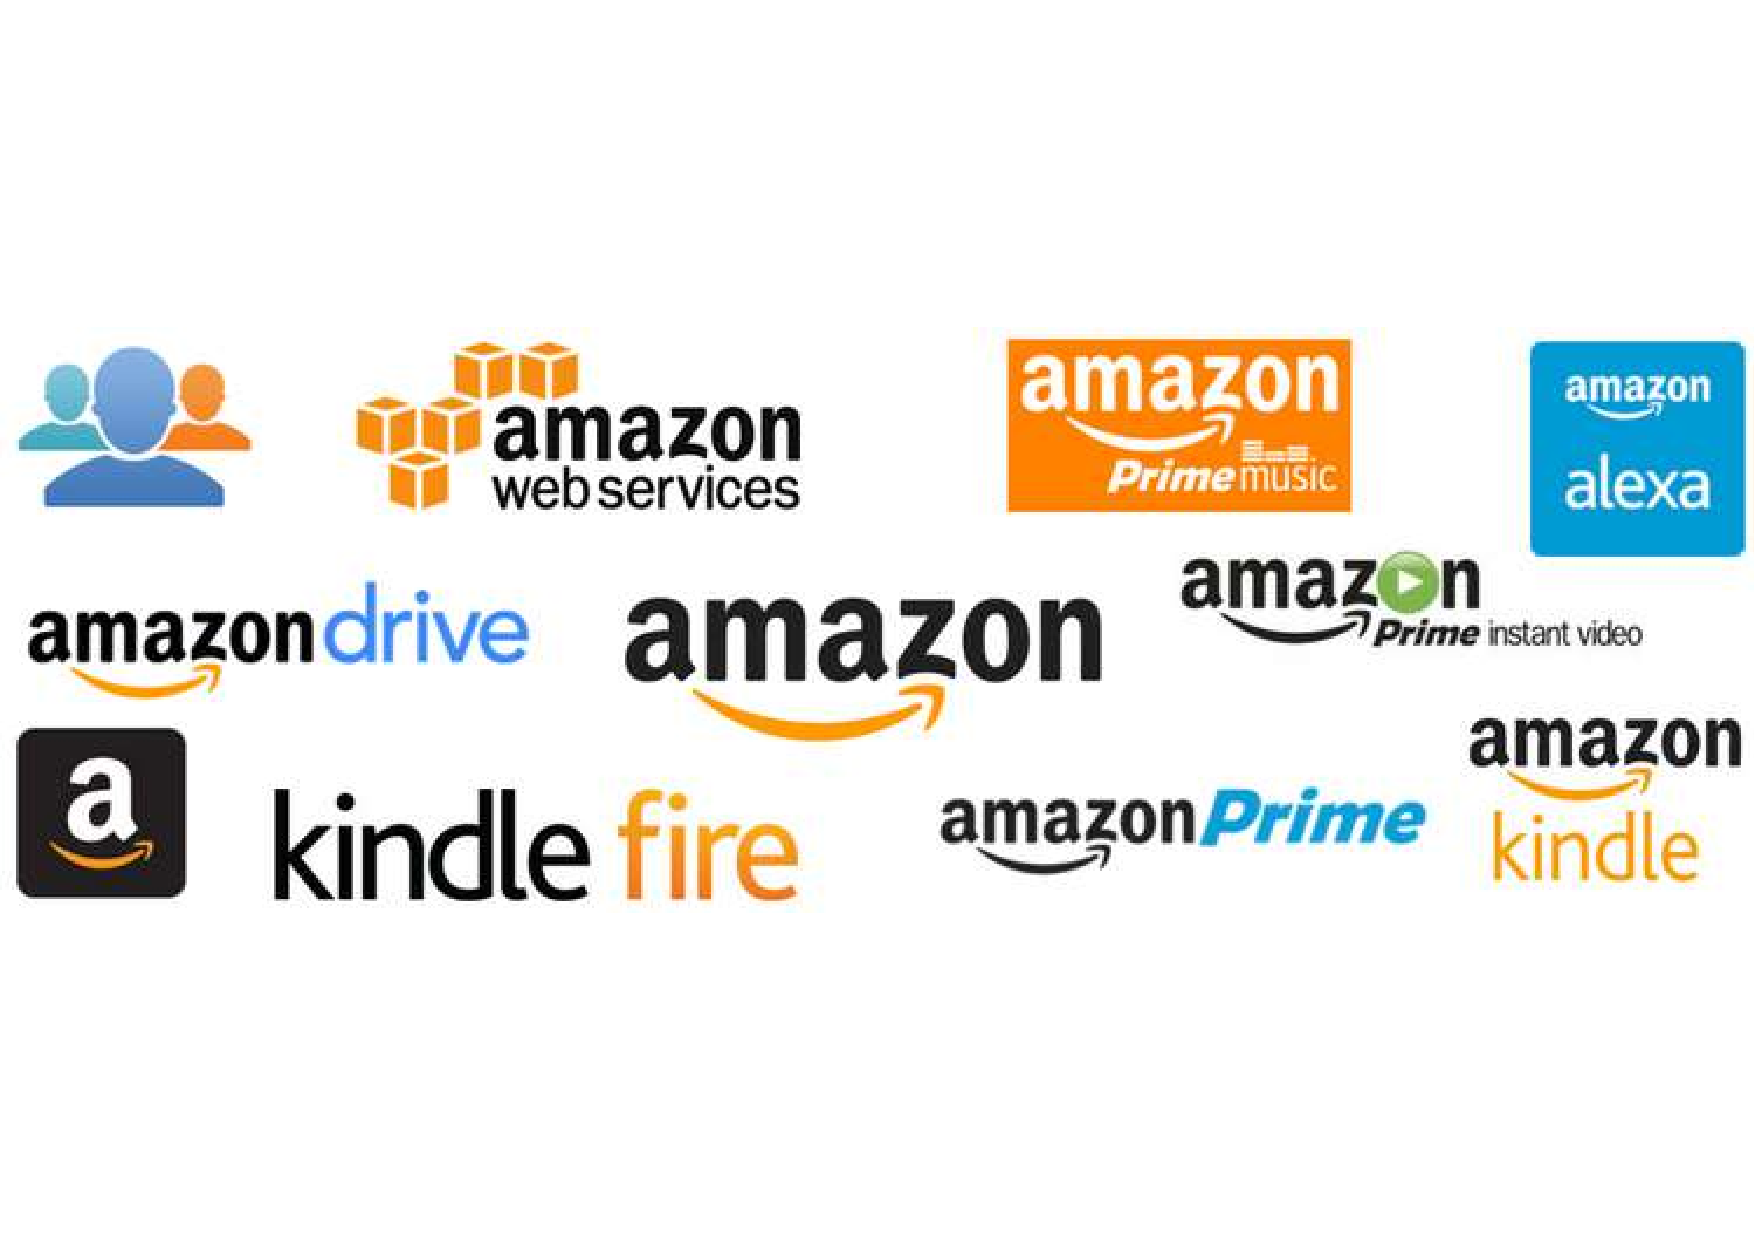
\includegraphics[width=0.8\linewidth]{./Graphismes-UTC/logos/Amazon/All-Things-Amazon.pdf}\hfill
        %\vspace{-1em}
        \caption{Les domaines d'activité d'Amazon}
    \end{figure}
En résumé, la structure diversifiée des services d'Amazon reflète ses compétences exceptionnelles dans la gestion de multiples facettes du commerce et de la technologie.


\subsubsection{Ses filiales en Europe}
\paragraph{}
\vspace{-2em}  % 减少1em的垂直空间
Amazon a solidement ancré ses activités à travers toute l'Europe, établissant des centres opérationnels, des entrepôts et des bureaux dans des pays clés tels que le Royaume-Uni, l'Allemagne, la France, l'Italie, l'Espagne et d'autres.
\paragraph{}
\vspace{-2em}  % 减少1em的垂直空间
Amazon a diversifié ses activités en Europe à travers différentes filiales spécialisées. Par exemple, Amazon Web Services (AWS) offre des services cloud, tandis que des entités comme Amazon Prime se concentrent sur les services de streaming et la livraison rapide.
\paragraph{}
\vspace{-2em}  % 减少1em的垂直空间
L'Europe a également été le terrain d'innovations majeures pour Amazon, notamment dans le domaine de l'intelligence artificielle, de l'automatisation des entrepôts et du développement de solutions technologiques avancées pour améliorer l'expérience client.
\paragraph{}
\vspace{-2em}  % 减少1em的垂直空间
La filiale française du groupe est ouverte en 2000. En 2016, Amazon devient le premier distributeur non alimentaire en France par le chiffre d'affaires.

\begin{figure}[htbp]
    \centering
    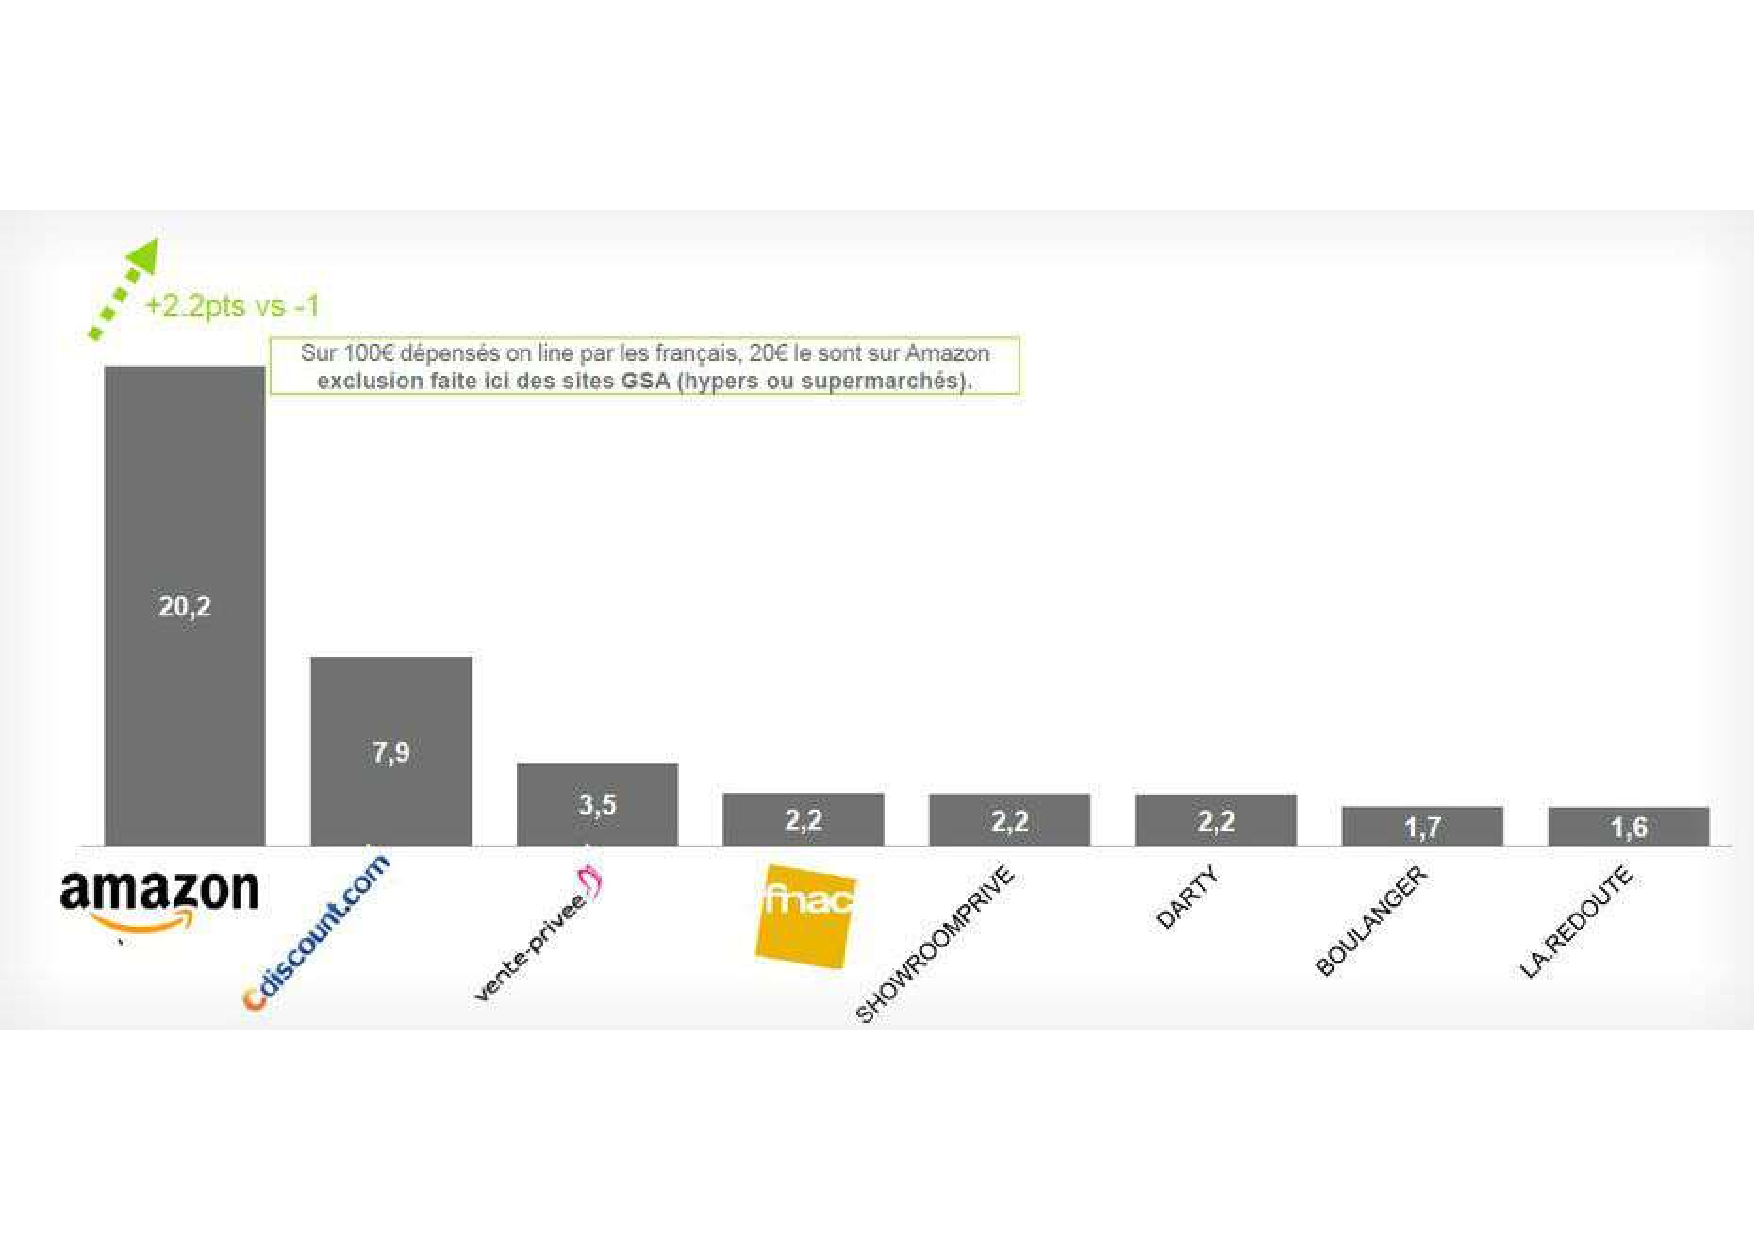
\includegraphics[width=0.8\linewidth]{./Graphismes-UTC/logos/Amazon/000315176_illustration_large.pdf}\hfill
    %\vspace{-1em}
    \caption{La comparaison entre Amazon et les autres plateformes en France}
\end{figure}
La présence d'Amazon en Europe a eu un impact significatif sur l'économie de la région, générant des emplois directs et indirects, stimulant le commerce local.
Amazon a également pris des engagements envers la durabilité environnementale en Europe, en investissant dans des initiatives d'énergies renouvelables et en travaillant à atteindre des objectifs de neutralité carbone.

\subsubsection{Son statut au marché}

\paragraph{}
\vspace{-2em}  % 减少1em的垂直空间
Amazon occupe actuellement une position prédominante sur le marché mondial, définissant les normes dans divers secteurs économiques. En tant que leader incontesté du commerce électronique, l'entreprise détient une part de marché significative dans de nombreux pays, offrant une vaste gamme de produits et de services à des millions de clients. 

\paragraph{}
\vspace{-2em}  % 减少1em的垂直空间
Amazon Web Services (AWS) domine le marché du cloud computing, fournissant des solutions technologiques à des entreprises du monde entier. En matière de streaming et de divertissement, Amazon Prime Video rivalise avec les meilleures plates-formes, créant du contenu original et attirant un nombre croissant d'abonnés. L'acquisition de Whole Foods a consolidé sa présence dans le secteur alimentaire et de la distribution physique. La plateforme Marketplace continue de prospérer, permettant à des vendeurs tiers de profiter de l'infrastructure et de la clientèle d'Amazon. 

\paragraph{}
\vspace{-2em}  % 减少1em的垂直空间
Son statut au marché est également renforcé par sa capacité à anticiper et à s'adapter aux tendances, à investir dans l'innovation, et à maintenir une réputation solide en matière de service client. Dans l'ensemble, Amazon reste un acteur incontournable, influençant considérablement l'économie mondiale et redéfinissant continuellement les normes de l'industrie.

\paragraph{}
\vspace{-2em}  % 减少1em的垂直空间
L'évolution des chiffres d'affaires d'Amazon au fil des années est remarquable, reflétant une croissance soutenue et une expansion constante de ses activités. Depuis ses débuts en tant que librairie en ligne dans les années 1990, Amazon a connu une augmentation exponentielle de ses revenus, passant d'une entreprise de commerce électronique à une entité diversifiée offrant une multitude de services. Les chiffres d'affaires ont connu une croissance significative, alimentée par l'expansion de son catalogue de produits. En 2019, Amazon a réalisé un chiffre d'affaires de 280,5 milliards de dollars, contre 232,9 milliards de dollars en 2018.

\begin{figure}[htbp]
    %\begin{subfigure}{0.5\textwidth}
    \centering
    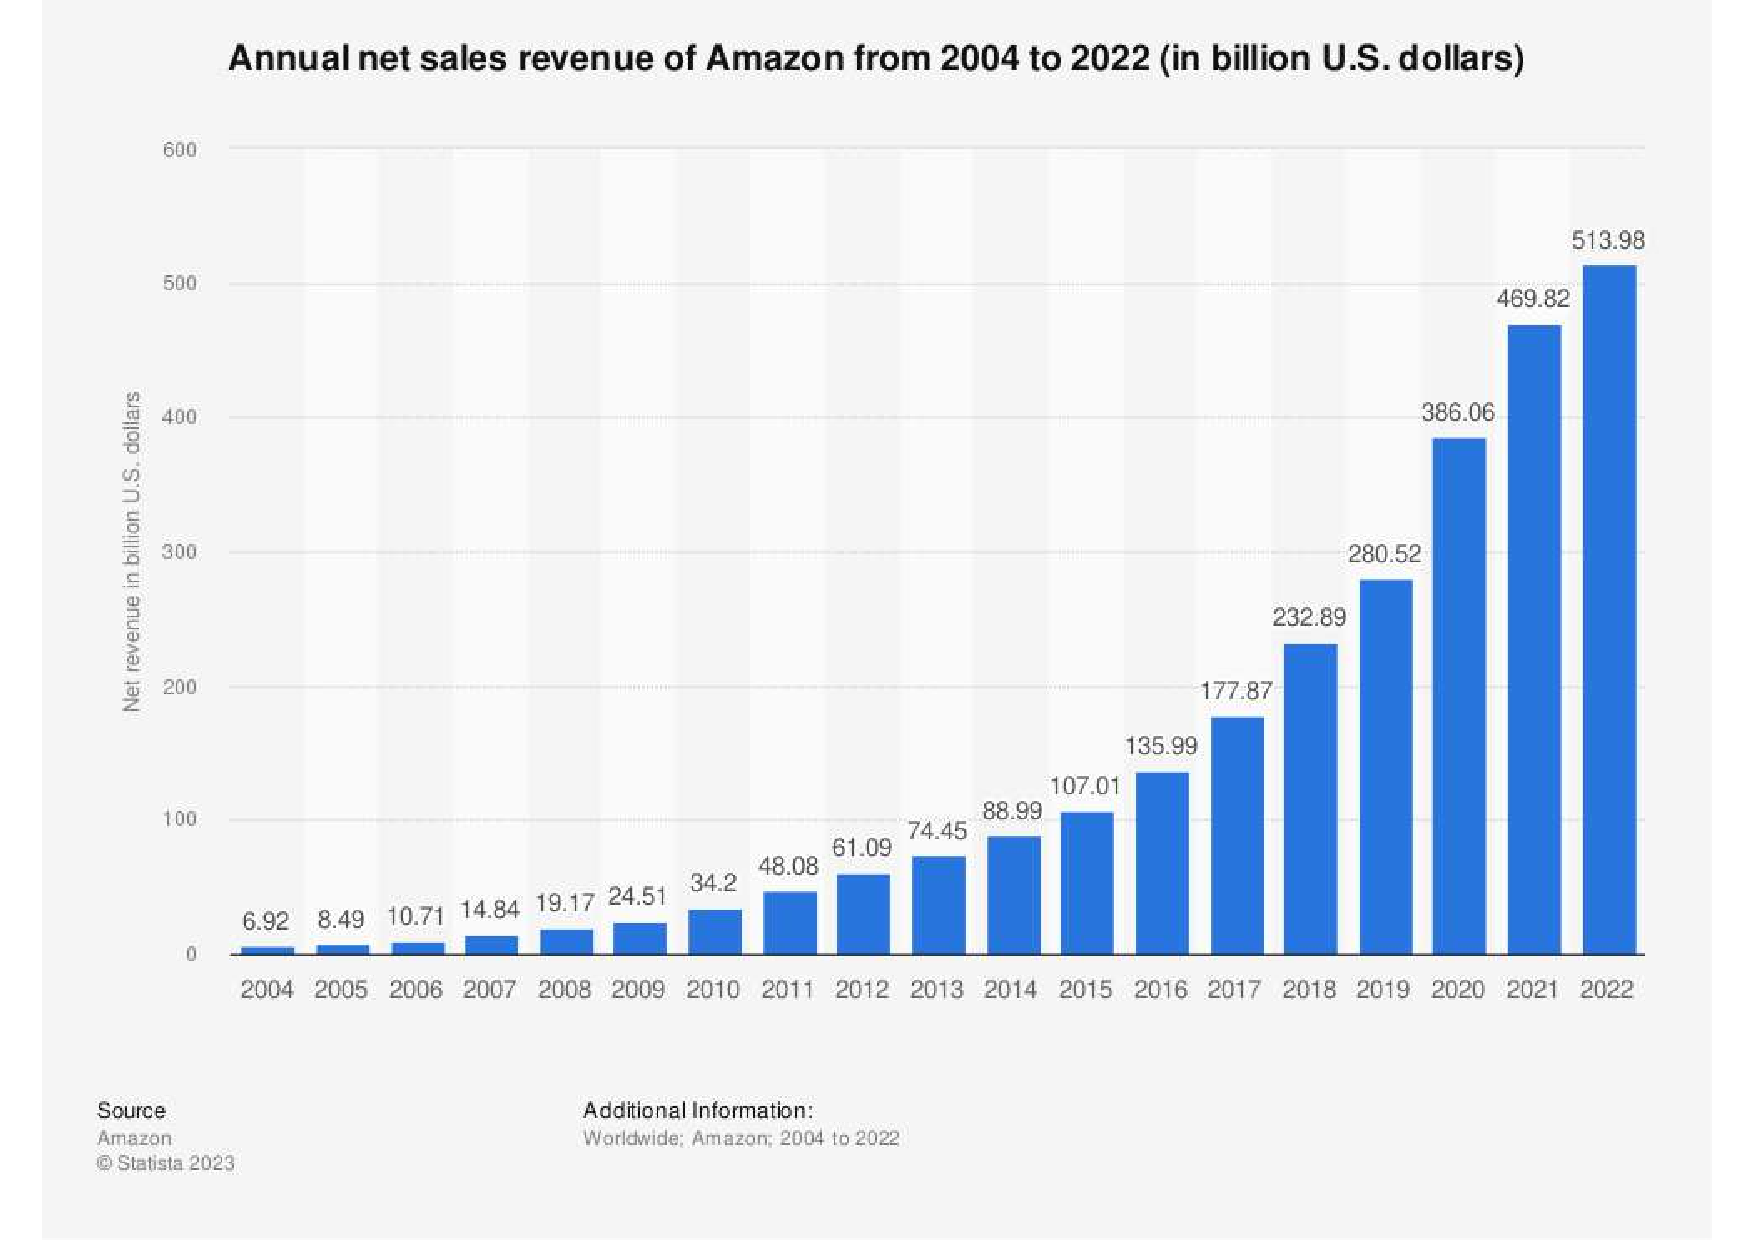
\includegraphics[width=0.8\linewidth]{./Graphismes-UTC/logos/Amazon/266282.pdf}\hfill
    %\vspace{-1em}
    \caption{L'évolution des chiffres d'affaires d'Amazon}
\end{figure}

\subsubsection{Ses impacts}
\paragraph{}
\vspace{-2em}  % 减少1em的垂直空间
Amazon est aujourd'hui devenu un acteur et un employeur engagé dans les territoires français. Dès sa création, Amazon n'a cessé d'innover en faveur d'une économie responsable, qui profite aux PME comme aux grandes entreprises sur l'ensemble du territoire. Amazon se mobilise également afin d'apporter sa contribution aux communautés locales proches de ses sites logistiques, à travers un soutien humain, matériel et financier, en particulier pour les personnes les plus démunies et durement touchées par la crise sanitaire actuelle.
\paragraph{}
\vspace{-2em}  % 减少1em的垂直空间

{\large\textbf{Croissance économique}}
\paragraph{}
\vspace{-3em}  % 减少1em的垂直空间
Depuis deux décennies, Amazon a noué une relation forte avec des dizaines de millions de clients qui la font confiance et apprécient l'apport d'Amazon à leur qualité de vie et à leur pouvoir d'achat. Pour mieux les servir, Amazon a investi plus de 11 milliards d'euros dans nos activités françaises entre 2010 et 2020. Grâce à ces investissements, Amazon est devenu l'un des principaux créateurs d'emplois en France et emploie 15 500 salariés en CDI en France.
\paragraph{}
\vspace{-2em}  % 减少1em的垂直空间

{\large\textbf{Soutien à l'entrepreneuriat}}
\paragraph{}
\vspace{-3em}  % 减少1em的垂直空间
Amazon propose des outils et des ressources pour aider les petites et moyennes entreprises, les auteurs, les clients AWS, et les partenaires de livraison à développer leur activité. Ils peuvent ainsi être au service de leur territoire, tout en offrant plus de choix aux clients du monde entier.
\paragraph{}
\vspace{-2em}  % 减少1em的垂直空间
En plus, Amazon accompagne le succès des petites et moyennes entreprises françaises: elles ont créé plus de 25 000 emplois en France pour soutenir leur activité en ligne.
\paragraph{}
\vspace{-2em}
L'an dernier, les petites et moyennes entreprises (PME) françaises ont vendu plus de 55 millions de produits dans les boutiques Amazon. En moyenne, elles vendent plus de 100 produits par minute dans les boutiques.
\paragraph{}
\vspace{-2em}  % 减少1em的垂直空间

{\large\textbf{Impact à l'échelle locale}}
\paragraph{}
\vspace{-3em}  % 减少1em的垂直空间
Amazon est aujourd'hui devenu un acteur et un employeur engagé dans les territoires français. En effet, Amazon se mobilise afin d'apporter sa contribution aux territoires et communautés dans lesquels les sites logistiques sont implantés, en mobilisant sa capacité à innover rapidement mais également à travers un soutien humain, matériel et financier.
\paragraph{}
\vspace{-2em}  % 减少1em的垂直空间
Amazon travaille en étroite collaboration avec des partenaires pour trouver des solutions aux enjeux mondiaux les plus pressants, en créant notamment des programmes innovants, qui laisseront une empreinte durable et positive.
Partout en France, Amazon accompagne les populations locales en veillant notamment à ce que les jeunes, dans le cadre du programme Amazon Future Engineer, soient sensibilisés aux opportunités et métiers du numérique et ce dès le plus jeune âge. Amazon se mobilise également pour que leurs besoins essentiels soient couverts.

\subsubsection{Ses concurrents}

\paragraph{}
\vspace{-2em}  % 减少1em的垂直空间
Amazon opère dans un environnement commercial concurrentiel où plusieurs entreprises cherchent à rivaliser dans des secteurs spécifiques. 

\paragraph{}
\vspace{-2em}  % 减少1em的垂直空间
Dans le domaine du commerce électronique, des concurrents tels qu'eBay et Alibaba se positionnent en tant que forces importantes, chacun avec des approches distinctes. Alibaba, par exemple, domine le marché chinois avec une présence mondiale croissante. En ce qui concerne le cloud computing, Microsoft Azure et Google Cloud sont des concurrents majeurs d'Amazon Web Services (AWS). La concurrence dans le secteur du streaming vidéo provient de sociétés telles que Netflix et Disney+. Dans le commerce alimentaire, des concurrents traditionnels tels que Walmart et des chaînes de supermarchés européennes jouent un rôle significatif. 
\paragraph{}
\vspace{-2em}  % 减少1em的垂直空间
Malgré cette concurrence féroce, Amazon maintient sa position dominante en raison de sa capacité à innover rapidement, à investir massivement dans la technologie, et à offrir une gamme diversifiée de services. La rivalité constante dans ces différents secteurs stimule l'innovation et incite Amazon à rester à l'avant-garde de l'évolution des marchés mondiaux.

\subsubsection{Son succès pendant la pandémie}
\paragraph{}
\vspace{-2em}  % 减少1em的垂直空间
La pandémie de coronavirus a entraîné la mort de plus d'un million de personnes dans le monde et a eu des répercussions dévastatrices sur l'économie mondiale, mettant certaines industries à l'arrêt, provoquant des licenciements massifs et accélérant le déclin des chaînes de grands magasins déjà en difficulté.
\paragraph{}
\vspace{-2em}  % 减少1em的垂直空间
Amazon, en tant que géant du commerce électronique, s'est démarqué comme l'une des rares exceptions. Offrant une vaste sélection et une recherche constante de commodité et de prix bas, il est devenu le détaillant par défaut et un service essentiel pour de nombreux consommateurs pendant la crise du coronavirus.

\paragraph{}
\vspace{-2em}  % 减少1em的垂直空间
Face à la fermeture des magasins et aux rayons vides, les consommateurs se sont tournés en masse vers Amazon pour des produits de protection tels que des désinfectants pour les mains, des masques et des désinfectants. Les ventes de produits ménagers et d'épicerie ont explosé, propulsant Amazon vers des ventes records au deuxième trimestre.

\paragraph{}
\vspace{-2em}  % 减少1em的垂直空间
Malgré des défis opérationnels initiaux, tels que des retards de livraison et des problèmes d'inventaire, Amazon a continué à embaucher massivement pour répondre à la demande croissante. Le PDG Jeff Bezos a souligné les difficultés rencontrées, mais Amazon prévoit de maintenir sa croissance pendant la saison des fêtes.

\paragraph{}
\vspace{-2em}  % 减少1em的垂直空间
Cependant, la pandémie a révélé des vulnérabilités dans la chaîne d'approvisionnement d'Amazon, perturbant son fonctionnement. La société continue de faire face à des problèmes d'inventaire, restreignant la quantité de marchandises stockées dans ses entrepôts.

\paragraph{}
\vspace{-2em}  % 减少1em的垂直空间
Malgré ces défis, Amazon prévoit de dépasser les 100 milliards de dollars de revenus trimestriels pour la première fois au quatrième trimestre, ce qui en ferait l'une des rares entreprises américaines à atteindre ce seuil aux côtés de Walmart et Exxon.

\subsection{Equipe}
\subsubsection{Mission}
\paragraph{}
\vspace{-2em}  % 减少1em的垂直空间
Notre équipe s'appelle \textit{Speed-Long term planning}. 
Notre objectif est de prendre les meilleures décisions pour nos clients et pour l'ensemble d'Amazon en nous basant sur les principaux indicateurs de performance (KPI) de l'entreprise : \textbf{Speed} (la promesse de livraison que nous voyons sur le site), \textbf{Delivery promise accuracy} (DEA, notre capacité à livrer à temps) et \textbf{Cost}. 
\paragraph{}
\vspace{-2em}  % 减少1em的垂直空间
Nous optimisons l'ensemble des opérations d'Amazon et les interactions entre ces métriques pour prendre les meilleures décisions de bout en bout. Notre vision est de réduire les coûts tout en maintenant une excellente expérience client grâce à la rapidité et à la DEA. Pour concrétiser cette vision, nous participons à la planification à long terme sur un horizon de 3 ans et à la planification opérationnelle à un an. Notre équipe est organisée en fonction des différentes activités d'Amazon (approvisionnement, expédition, placement, conception du réseau, ... ) et nous travaillons en étroite collaboration avec les équipes opérationnelles pour définir les objectifs et les plans d'action. Nous travaillons également avec les équipes techniques pour développer des outils et des modèles qui nous permettent de prendre des décisions basées sur des données et de les mettre en œuvre à grande échelle.
\paragraph{}
\vspace{-2em}  % 减少1em的垂直空间
Au sein de cette équipe, je rejoinds la sous-équipe \textit{Invenory} qui s'occupe des projets de placement des stocks (où et comment nous disposons les articles). Notre sous-équipe est composée de Marc, Matthieu, Francesca, Joy, Abhishek, Vinayak, et nous sommes tous sous la direction de Karan. 
\paragraph{}
\vspace{-2em}  % 减少1em的垂直空间
Dans notre équipe, la bienveillance est au cœur de notre culture. Nous encourageons l'échange ouvert d'idées, favorisons un esprit d'équipe solide et sommes là pour soutenir nos collègues.

\begin{figure}[htbp]
    %\begin{subfigure}{0.5\textwidth}
    \centering
    
\includegraphics[width=0.8\linewidth]{./Graphismes-UTC/logos/Amazon/equipe.pdf}\hfill
    %\vspace{-1em}
    \caption{Organigramme de notre sous-équipe \textit{Inventory}} 
\end{figure}



